\documentclass[letterpaper,12pt,twoside]{uncthesis}

\usepackage{pgfplots}
\usepackage{tikz}

\newcommand{\betrfs}{BetrFS\xspace}
\newcommand{\betrfsOne}{BetrFS 0.1\xspace}
\newcommand{\betrfsTwo}{BetrFS 0.2\xspace}
\newcommand{\betrfsThree}{BetrFS 0.3\xspace}
\newcommand{\betrfsFour}{BetrFS 0.4\xspace}
\newcommand{\bet}{B$^{\varepsilon}$-tree\xspace}
\newcommand{\bets}{B$^{\varepsilon}$-trees\xspace}
\newcommand{\btree}{B-tree\xspace}
\newcommand{\btrees}{B-trees\xspace}
\newcommand{\fti}{\textit{ft-index}\xspace}
\newcommand{\Fti}{\textit{Ft-index}\xspace}
\newcommand{\klibc}{\textbf{klibc}\xspace}
\newcommand{\mdb}{\texttt{meta\_db}\xspace}
\newcommand{\ddb}{\texttt{data\_db}\xspace}
\newcommand{\spre}{\textit{src\_prefix}\xspace}
\newcommand{\dpre}{\textit{dst\_prefix}\xspace}
\newcommand{\goto}{\texttt{GOTO}\xspace}
\newcommand{\delold}{\textit{del\_old}\xspace}
\newcommand{\bedag}{B$^{\varepsilon}$-DAG\xspace}
\newcommand{\bedags}{B$^{\varepsilon}$-DAGs\xspace}

\pgfkeys{
    /fs-names/ext4/.initial=ext4,
    /fs-names/btrfs/.initial=Btrfs,
    /fs-names/xfs/.initial=XFS,
    /fs-names/zfs/.initial=ZFS,
    /fs-names/nilfs2/.initial=NILFS2,
    /fs-names/betrfs3/.initial=\betrfsThree,
    /fs-names/betrfs3-max/.initial=\betrfsThree with one zone,
}

\pgfkeys{
    /fs-colors/ext4/.initial=blue,
    /fs-colors/btrfs/.initial=red,
    /fs-colors/xfs/.initial=green,
    /fs-colors/zfs/.initial=purple,
    /fs-colors/nilfs2/.initial=cyan,
    /fs-colors/betrfs3/.initial=orange,
    /fs-colors/betrfs3-max/.initial=black,
}

\pgfkeys{
    /fs-marks/ext4/.initial=triangle*,
    /fs-marks/btrfs/.initial=pentagon*,
    /fs-marks/xfs/.initial=square*,
    /fs-marks/zfs/.initial=diamond*,
    /fs-marks/nilfs2/.initial=o,
    /fs-marks/betrfs3/.initial=oplus,
    /fs-marks/betrfs3-max/.initial=+,
}

\newcommand{\addTokubenchZonePlot}[1]
{
    \addplot[
        color=\pgfkeysvalueof{/fs-colors/#1},
        line width=0.75pt,
        mark=\pgfkeysvalueof{/fs-marks/#1},
    ]
    plot[
    ]
    table[
    ]
    {./data/tokuzone/#1.csv};
    \addlegendentry{\pgfkeysvalueof{/fs-names/#1}}
}

\newtheorem{invariant}{Invariant}


%%%%%%%%%%%%%%%%%%%%%%%%%%%%%%%%%%%%%%%%%%%%%%%%%%%%%%%%%%%%
% Required thesis information
%%%%%%%%%%%%%%%%%%%%%%%%%%%%%%%%%%%%%%%%%%%%%%%%%%%%%%%%%%%%

% When indicating your degree in the second bracketed space, use the full
% degree name (i.e., Doctor of Philosophy, not Ph.D. or PHD; Master of Public
% Health, not M.P.H. or MPH; Master of Social Work, not M.S.W. or MSW).
\uncdegreename{Doctor of Philosophy}

% List your department, school, or curriculum rather than your subject area or
% specialty discipline in the third bracketed space. You may include your
% subject area or specialty discipline in parentheses (i.e., Department of
% Romance Languages (French); School of Pharmacy (Molecular Pharmaceutics);
% School of Education (School Psychology); or similar official area).
% If you wish to include both your department and school names, list the school
% at the end of the statement (i.e., Department of Pharmacology in the School
% of Medicine).
\uncthesisdepartment{Department of Computer Science}

% Type can be dissertation or thesis
\uncthesistype{dissertation}

% Title
\uncthesistitle{Efficient, Locality-Maintaining Namespace Operations in a Write-Optimized File System}

% Name
\uncthesisauthor{Yang Zhan}

% University Name
\uncthesisuniversity{University of North Carolina at Chapel Hill}

% The year in which your committee approves the completed thesis or
% dissertation. This need not be the year you graduate.
\uncthesisyear{2019}

% Thesis advisor. Appears on the abstract page.
\uncthesisadvisor{Donald E. Porter}

% Thesis committee. Appears on the title page.  Do not include titles such as
% Professor, Doctor, Dr., PhD, or any identifiers such as “chair” or “advisor”
% before or after any names.  Put a new line after each name to render
% correctly on title page.
\uncthesiscommittee{Donald E. Porter\\
Leonard McMillan\\
F. Donelson Smith\\
Rob Johnson\\
Ethan L. Miller
}

%%%%%%%%%%%%%%%%%%%%%%%%%%%%%%%%%%%%%%%%%%%%%%%%%%%%%%%%%%%%
% Font selection
%%%%%%%%%%%%%%%%%%%%%%%%%%%%%%%%%%%%%%%%%%%%%%%%%%%%%%%%%%%%
% Font, if using PDFLaTeX
\usepackage{times}
% Font, if using XeLaTeX
%\usepackage{fontspec}
%\setmainfont{Times New Roman}

% Prevent awkward hyphenations.
\hyphenation{Raj-kumar}

\begin{document}
% The following order of the contents is REQUIRED
\pagenumbering{roman}


% 1. Title Page
\input{template/frontmatter/1_titlepage}

% 2. Copyright Page (optional)
%\newgeometry{left=\uncthesisleftmargin in,top=8.42in,right=\uncthesisrightmargin in,bottom=1in,nohead}

\begin{center}
\begin{singlespace}
\copyright~\uncthesisyear\\
\uncthesisauthor \\
ALL RIGHTS RESERVED
\end{singlespace}
\end{center}

\clearpage
\newgeometry{left=\uncthesisleftmargin in,top=2in,right=\uncthesisrightmargin in,bottom=1in,nohead}
% Normal pages from here on out; TOC title takes care of 2in requirement.
\restoregeometry


% 3. Abstract
\begin{abstract}

Good locality and efficient namespace operations are considered mutually
exclusive in a file system.
Traditional inode-based file systems have good rename performance, but fail
to maintain locality, especially in the face of file system aging.
On the other hand, full-path-indexed file systems ensure locality, however,
renaming a directory needs to update all related full-paths,
which is usually implemented as an expensive operation.

This dissertation describes a technique that has both good locality and
efficient namespace operations.
In particular, we describe a novel synthesis of write-optimization,
full-path indexing and operations on data structures.
By directly manipulating the data structure, a full-path-indexed file system
can efficiently update related full-paths in a rename.
Moreover, with the technique, a full-path-indexed file system can
clone a directory without traversing the directory.

We implement this technique in \betrfs, a full-path-indexed, write-optimized,
local file system for Linux.
Compared to ext4, the widely used inode-based file system in Linux,
the new version of \betrfs traverses the Linux source directory 9.47x faster,
and renames the same directory 1.09x faster.
Meanwhile, the new version of \betrfs clones a directory faster than
file systems that clone the directory through file clones,
such as Btrfs and XFS.

\end{abstract}


% 4. Dedication, Acknowledgement(s), Preface (each optional)
%\begin{dedication}
A dedication is a message from the author prefixed to a work in tribute to a person, group, or cause. Most dedications are short statements of tribute beginning with \textit{``To \ldots''} such as \textit{``To my family''}.
\end{dedication}

%\begin{acknowledgement}

Acknowledgements are the author's statement of gratitude to and recognition of the people and institutions that helped the author's research and writing.

    \lipsum[5]
\end{acknowledgement}

%\begin{preface}

A preface is a statement of the author's reasons for undertaking the work and other personal comments that are not directly germane to the materials presented in other sections of the thesis or dissertation. These reasons tend to be of a personal nature.

    \lipsum[6]

\end{preface}


% 5. Table of Contents, with page references
\input{template/frontmatter/5_toc}

% 6. List of Tables, with titles and page references (if applicable). And list
% of Figures or Illustrations, with titles and page references (if applicable)
\input{template/frontmatter/6_lot}
\input{template/frontmatter/6_lof}

% 7. List of Abbreviations (if applicable)
%\phantomsection
\addcontentsline{toc}{chapter}{LIST OF ABBREVIATIONS}

\begin{center}
\textbf{LIST OF ABBREVIATIONS}
\vspace{16pt}
\end{center}

% TODO: define new column types to make sure multi-line table cells has single-spacing

\noindent
\begin{tabular}{p{0.8in} p{5in}}
CoS     & Chamber of Secrets\\
DA      & Dumbledore's Army\\
DADA    & Defence Against the Dark Arts\\
DH      & Deathly Hallows \\
FBAWTFT & Fantastic Beasts and Where to Find Them\\
SPEW    & Society for the Protection of Elvish Welfare\\
VWI     & Voldemort War One\\
VWII    & Voldemort War Two\\
\end{tabular}

\clearpage


% 8. List of Symbols (if applicable)
%\phantomsection{}
\addcontentsline{toc}{chapter}{LIST OF SYMBOLS}

\begin{center}
\textbf{LIST OF SYMBOLS}
\vspace{16pt}
\end{center}

\noindent
\begin{tabular}{@{}p{0.8in} l}
$M$ & Number of wands\\
$m$ & Number of wizards\\
$n$ & Number of fantastic beasts\\
\end{tabular}

\clearpage


\pagenumbering{arabic}

%\chapter{Formatting Guide}
\label{chap:formatting_guide}

\section{Margins}

This template follows the UNC graduate school thesis/dissertation formatting guide as rigidly as possible.
This template has uniform margins throughout the entire document:
\begin{itemize}
    \item Left: 1''
    \item Right: 1''
    \item Top: 1''
    \item Bottom: 1''
\end{itemize}

\section{Font}
A TrueType font is recommended/required by the ProQuest dissertation publishing. Recommended fonts and sizes can be found in \autoref{tab:font}.

\begin{table}
    \centering
    \caption{Recommended font type and size}\label{tab:font}
    \begin{tabular}{ll}
        \toprule
        Font name            & Font Size \\ \midrule
        Arial                & 10pt\\
        Century              & 11pt\\
        Courier New          & 10pt\\
        Garamond             & 12pt\\
        Georgia              & 11pt\\
        Lucida Bright        & 10pt\\
        Microsoft Sans Serif & 10pt\\
        Tahoma               & 10pt\\
        Times New Roman      & 12pt\\
        Trebuchet MS         & 10pt\\
        Verdana              & 10pt\\ \bottomrule
    \end{tabular}
\end{table}

If you're using \texttt{pdflatex} to compile this template, include the \texttt{times} package in the preamble.
If you're using \texttt{xelatex} to compile this template, you can use the \texttt{fontspec} package and the \texttt{setmainfont} command to choose your favorite font.
This template by default uses 12pt Times New Roman.

\section{Spacing and Indentation}

The template takes care of spacing and indentation:
\begin{itemize}
    \item Text appears in a single column on each page and is double-spaced throughout the document.
    \item New paragraphs are indicated by a consistent tab indentation throughout the entire document.
    \item The document text is left-justified.
    \item For blocked quotations, indent the entire text of the quotation consistently from the left margin.
\end{itemize}

\lipsum[6]
\begin{quote}
    This is an example showing the indentation of block quoted text.
    \lipsum[8]
\end{quote}
\lipsum[7]

\section{Pagination}
This template takes care of pagination.

Pagination and margin are also well maintained for landscape pages.
\begin{landscape}
    \lipsum[9] Let's also see how does footnote works in landscape pages~\footnote{We have a footnote in landscape environment}.
\end{landscape}

\section{Footnotes and Endnotes}
Footnotes\footnote{\lipsum[10]} and endnotes\footnote{\lipsum[11]} obey the
formatting guide. However, using both of them confuses the note numbering.
Given the discrepancy between the official format guide\endnote{\lipsum[12]}
and the official sample pages\endnote{\lipsum[14]}, the correct order for
endnotes and appendixes are unclear.  Thus, using only footnote is recommended.

\section{Tables and Figures}
Tables, figures, and illustrations vary widely by discipline. Therefore, formatting of these
components is largely at the discretion of the author.

List of figures and list of tables are well taken care of by \LaTeX{} and this
template.  If an entry in LOT/LOF takes up more than one line, break up the
entry about three-fourths of the way across the page and place the rest of the
text on a second line, single-spacing the two lines.

One nice trick is the short caption option for the
\texttt{\textbackslash{}caption{}} command.  It allows the LOT/LOF only include
the short caption but not the full caption.
\begin{figure}
    \centering
    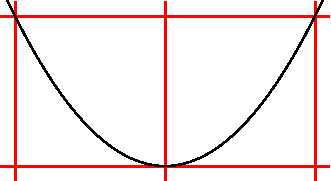
\includegraphics[width=0.5\textwidth]{figures/demo.pdf}
    \caption{A very long caption that does not make much sense but only tests the line-breaking and line-spacing in LOT/LOF.}
\end{figure}

\begin{figure}
    \centering
    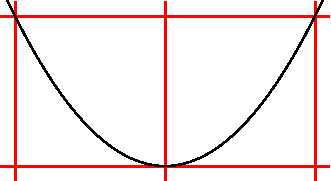
\includegraphics[width=0.5\textwidth]{figures/demo.pdf}
    \caption[Short Caption]{A very long caption that does not make much sense but only tests the line-breaking and line-spacing in LOT/LOF.}
\end{figure}

\section{Reference}
The APA style is used for references. Notice the differences caused by different citation command.

\begin{table}
    \centering
    \caption[Short title]{Comparison of different citation command.}\label{tab:citation}
    \begin{tabular}{ll}
        \toprule
Command                        & Results \\ \midrule
\texttt{\textbackslash{}cite}  & \cite{LFR}\\
\texttt{\textbackslash{}citep} & \citep{LFR}\\
\texttt{\textbackslash{}citet} & \citet{LFR}\\\bottomrule
    \end{tabular}
\end{table}

\section{Length}
There are no requirements for the length of the PhD thesis. For the Department of Computer Science, from 2014 to 2017, average length of the thesis main body text is $\mu \approx 120, \sigma \approx 33$, average length of main body text + reference is $\mu \approx 129, \sigma \approx 35$.
%\chapter{Related Works}
\label{chap:related}

\section{A very long section title testing the line-breaking and line-spacing in TOC if not long enough we make it longer}
\subsection{Subsection title}
\lipsum{}
\subsubsection{Subsubsection title}
\lipsum[1]
\subsection{Another subsection title}


\chapter{Introduction}
\label{chap:intro}

Today's general purpose file systems fail to utilize the full bandwidth of the
underlying hardware.
Widely used inode-based file systems, such as ext4, XFS, and Btrfs, can write
large files at near disk bandwidth,
but typically create small files at less than 3\% of the disk bandwidth.
Similarly, these file systems can read large files at near disk bandwidth,
but scanning directories with many small files is slow, and the performance
degrades when the file system ages~\citep{betrfs3}.

At the heart of this issue is how data is organized on disk.
The most common design pattern for modern file systems is to use multiple layers
of indirection.
The inode number of a file or directory connects the name of an entry in a
directory to its metadata location on disk.
The metadata of an inode contains extents that describes the physical location
and length of data at different offsets.
Indirection simplifies implementation of the file system, and makes some
operations, such creating files and appending files, easy to implement.
In particular, namespace operations are simple and flexible.
For example, a rename is just a pointer swing, moving an entry from one
directory to another directory.
However, indirection doesn't impose any constraint on how metadata and data
are placed on the disk.
In the worst case, the metadata of entries under a directory and the content of
a file can end up scattered over the disk.
Heuristics, such as cylinder groups~\citep{ffs1}, are designed to mitigate this
problem.
However, on modern inode-based file systems, unless the metadata or data are
modified, their location doesn't change.
Therefore, after disk space is allocated and freed over file system aging,
the free space on disk becomes scattered,
leading to bad performance for both reads and writes.

One attempt to solve the problem of random writes is the log-structured file
system~\citep{lfs}.
The log-structure file system treats the disk as a log, so small random writes
becomes log appends, which are significantly faster.
However, the log cleaner in a log-structured file system has severe impact on
performance~\citep{lfsbsd}, especially when the log is full.
And the log-structured file system still uses multiple levels of
indirection, resulting in slow directory traversals.

An alternative design is to use full-path indexing upon write-optimized
dictionaries (WODs) in a file system, known to have good performance on nearly
all operations.
On one hand, WODs have fast random write performance.
A WOD divides its data into multiple levels whose sizes grow exponentially.
Writes are put to the lowest level, and gradually merged to higher levels in
batches.
This merging process in a WOD keeps data sorted in a certain order at each level
and acts as a cleaner to garbage-collect lower levels.
On the other hand, full-path indexing ensures metadata and data in
depth-first-search order, that is, lexicographic order by the full-path names
of files and directories.
With full-path indexing, metadata and data under one directory are close to each
other in key space, which, combined with the sorted order maintained by
WODs, leads to good locality and fast directory traversals.
Prior work~\citep{betrfs1,betrfs1tos,betrfs2,betrfs2tos,betrfs3} of this design
realizes efficient implementation of many file-system operations, such as random
writes, file creates and directory traversals,
but a few operations still have prohibitively high overheads.

The Achilles' heel of such design is the performance of namespace operations,
in particular, renaming large files and directories.
For instance, renaming a large directory changes the full-paths of all files
and directories under it, which updates keys of the metadata and
data and moves them in the key space.
Competitive performance for namespace operations in full-path-indexed file
systems should complete in an I/O-efficient manner.

However, prior work mainly focuses on the schema level of the file system, i.e.,
how metadata and data are keyed and indexed in the WODs.
The full-path-indexed file system usually implements a rename by
fetching all key/value pairs of metadata and data,
inserting them back with updated keys, and deleting old key/value pairs.
Therefore, a rename needs to call several operations for each affected full-path
names, leading to bad performance.
Or, the file system partly backs away from full-path-indexing and adopts
relative-path-indexing, a hybrid of full-path-indexing and indirection.
This approach not only breaks the locality of full-path-indexing, but also
taxes other operations for efficient namespace operations.

This dissertation presents I/O-efficient ways to do namespace operations in a
full-path-indexed, write-optimized file system.
Specifically, though full-path indexing limits possible change on the schema
level, we observe that it can make all full-path names under a directory
contiguous in key space.
And the underlying WOD, \bets, has a tree structure, which makes it possible to
move or clone a contiguous key range efficiently.
Therefore, we dig into the underlying \bets, and implements two new operations,
range-rename and range-clone, that completes file system renames and clones with
bounded number of I/Os.

Chapter~\ref{chap:bg} talks about the necessary background of this dissertation.
We start with a presentation of the write-optimized \bets,
showing the idea of write-optimization.
Then, we describes full-path-indexed \betrfs and relative-path-indexed \betrfs.
The full-path-indexed \betrfs shows the benefit of full-path indexing combined
with write-optimization, but suffers from slow renames.
The relative-path-indexed \betrfs has good rename performance, but breaks the
full-path indexing and taxes other operations for efficient renames.

Chapter~\ref{chap:rename} presents the range-rename operation on \bets,
which full-path-indexed \betrfs can use to implement file system renames.
A range-rename updates all keys with one prefix to another prefix efficiently
through two techniques, \textbf{key lifting} and \textbf{tree surgery}.

Chapter~\ref{chap:clone} expands range-rename to range-clone,
which full-path-indexed \betrfs can use to implement both file or directory
renames and clones.
We first show how to implement range-clone with range-rename techniques by
transforming \bets into \bedags.
Then, we introduces a new type of messages, \goto messages, that works as other
messages in \bedags, fitting range-clone into write-optimization.

Chapter~\ref{chap:eval} evaluates the implementation.
We compare full-path-indexed \betrfs with range-rename or range-clone to
widely used file systems on micro and application benchmarks.
We also put a particular focus on benchmarking the range-rename and range-clone
operations.

Chapter~\ref{chap:related} summarize some previously published work related to
this work.
We organize related work by topic, and talk in detail about work that is closely
related to this work.

Chapter~\ref{chap:conclusion} summarizes and concludes the dissertation.

The primary contribution of this dissertation is to show that there is no
trade-off between efficient namespace operations and locality.
Efficient renames are possible in a full-path-indexed file system, which ensures
locality.
And full-path indexing creates more opportunities for namespace operations,
such as directory clones.



\chapter{Background}
\label{chap:bg}

This chapter gives the background of \betrfs~\citep{betrfs1,betrfs1tos,betrfs2,betrfs2tos,betrfs3}.
\betrfs is a file system based on write-optimized \bets.
Also, \betrfs adopts full-path indexing or relative-path indexing for locality.

Section~\ref{sec:bg:bet} introduces the underlying data structure in \betrfs,
the \bet.
The \bet is a WOD that treats writes as messages and cascades messages in
batches.
Then, Section~\ref{sec:bg:fpi} describes full-path-indexed \betrfs.
Full-path indexing keeps metadata and data under one directory close to each
other in the key space,
but makes the simple implementation of file system renames expensive.
Next, Section~\ref{sec:bg:rpi} discusses relative-path indexing,
the previous approach that taxes other operations to mitigate the rename issue
in \betrfs.
At last, Section~\ref{sec:bg:impl} talks about implementation details
in \betrfs.

\section{\bets}
\label{sec:bg:bet}

\bets~\citep{bet,betlogin} are \btrees, augmented with buffers in non-leaf
nodes.
New writes are injected as messages into the buffer of the root node of a \bet.
When a node's buffer becomes full, messages are flushed from that node's buffer
to one of its children.
If the child is a non-leaf node, messages are injected into the child's
buffer.
Otherwise, messages take effect on the leaf node.
An insert message becomes a key/value pair in the leaf node.
If there is an old/key/value pair with the same key in the leaf node,
the insert message overwrites the old/key value pair;
A delete message removes the old key/value pair with the same key in the leaf
node.
Therefore, in a \bet, leaf nodes only store key/value pairs, as in a \btree.
Because writes can be messages in non-leaf nodes, point and range queries on a
\bet must check the buffers along the root-to-leaf path,
as well as key/value pairs in leaf nodes.

\begin{figure}[t]
    \centering
    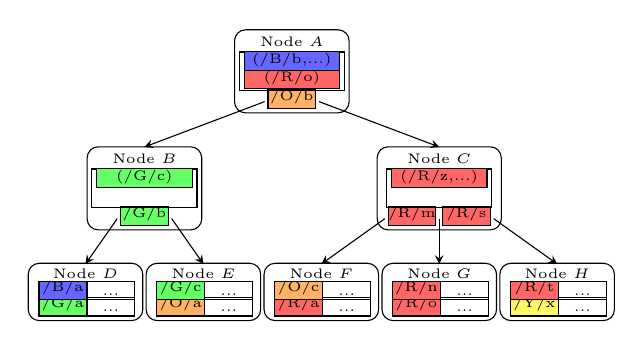
\begin{tikzpicture}[xscale=0.95, yscale=0.95]
        \node[anchor=south, rectangle, rounded corners, minimum height=.06\textwidth, minimum width=.12\textwidth, draw=black] at (0, 0) {};
        \node[anchor=south, font=\tiny] at (0, .036\textwidth) {Node $F$};
        \node[anchor=south, rectangle, minimum height=.015\textwidth, minimum width=.05\textwidth, draw=black, fill={red!60}] at (-.025\textwidth, .005\textwidth) {};
        \node[anchor=south, font=\tiny] at (-.025\textwidth, 0) {/R/a};
        \node[anchor=south, rectangle, minimum height=.015\textwidth, minimum width=.05\textwidth, draw=black] at (.028\textwidth, .005\textwidth) {};
        \node[anchor=south, font=\tiny] at (.028\textwidth, 0) {...};
        \node[anchor=south, rectangle, minimum height=.015\textwidth, minimum width=.05\textwidth, draw=black, fill={orange!60}] at (-.025\textwidth, .023\textwidth) {};
        \node[anchor=south, font=\tiny] at (-.025\textwidth, .018\textwidth) {/O/c};
        \node[anchor=south, rectangle, minimum height=.015\textwidth, minimum width=.05\textwidth, draw=black] at (.028\textwidth, .023\textwidth) {};
        \node[anchor=south, font=\tiny] at (.028\textwidth, .018\textwidth) {...};

        \node[anchor=south, rectangle, rounded corners, minimum height=.06\textwidth, minimum width=.12\textwidth, draw=black] at (.13\textwidth, 0) {};
        \node[anchor=south, font=\tiny] at (.13\textwidth, .036\textwidth) {Node $G$};
        \node[anchor=south, rectangle, minimum height=.015\textwidth, minimum width=.05\textwidth, draw=black, fill={red!60}] at (.105\textwidth, .005\textwidth) {};
        \node[anchor=south, font=\tiny] at (.105\textwidth, 0) {/R/o};
        \node[anchor=south, rectangle, minimum height=.015\textwidth, minimum width=.05\textwidth, draw=black] at (.158\textwidth, .005\textwidth) {};
        \node[anchor=south, font=\tiny] at (.158\textwidth, 0) {...};
        \node[anchor=south, rectangle, minimum height=.015\textwidth, minimum width=.05\textwidth, draw=black, fill={red!60}] at (.105\textwidth, .023\textwidth) {};
        \node[anchor=south, font=\tiny] at (.105\textwidth, .018\textwidth) {/R/n};
        \node[anchor=south, rectangle, minimum height=.015\textwidth, minimum width=.05\textwidth, draw=black] at (.158\textwidth, .023\textwidth) {};
        \node[anchor=south, font=\tiny] at (.158\textwidth, .018\textwidth) {...};

        \node[anchor=south, rectangle, rounded corners, minimum height=.06\textwidth, minimum width=.12\textwidth, draw=black] at (.26\textwidth, 0) {};
        \node[anchor=south, font=\tiny] at (.26\textwidth, .036\textwidth) {Node $H$};
        \node[anchor=south, rectangle, minimum height=.015\textwidth, minimum width=.05\textwidth, draw=black, fill={yellow!60}] at (.235\textwidth, .005\textwidth) {};
        \node[anchor=south, font=\tiny] at (.235\textwidth, 0) {/Y/x};
        \node[anchor=south, rectangle, minimum height=.015\textwidth, minimum width=.05\textwidth, draw=black] at (.288\textwidth, .005\textwidth) {};
        \node[anchor=south, font=\tiny] at (.288\textwidth, 0) {...};
        \node[anchor=south, rectangle, minimum height=.015\textwidth, minimum width=.05\textwidth, draw=black, fill={red!60}] at (.235\textwidth, .023\textwidth) {};
        \node[anchor=south, font=\tiny] at (.235\textwidth, .018\textwidth) {/R/t};
        \node[anchor=south, rectangle, minimum height=.015\textwidth, minimum width=.05\textwidth, draw=black] at (.288\textwidth, .023\textwidth) {};
        \node[anchor=south, font=\tiny] at (.288\textwidth, .018\textwidth) {...};

        \node[anchor=south, rectangle, rounded corners, minimum height=.06\textwidth, minimum width=.12\textwidth, draw=black] at (-.13\textwidth, 0) {};
        \node[anchor=south, font=\tiny] at (-.13\textwidth, .036\textwidth) {Node $E$};
        \node[anchor=south, rectangle, minimum height=.015\textwidth, minimum width=.05\textwidth, draw=black, fill={orange!60}] at (-.155\textwidth, .005\textwidth) {};
        \node[anchor=south, font=\tiny] at (-.155\textwidth, 0) {/O/a};
        \node[anchor=south, rectangle, minimum height=.015\textwidth, minimum width=.05\textwidth, draw=black] at (-.102\textwidth, .005\textwidth) {};
        \node[anchor=south, font=\tiny] at (-.102\textwidth, 0) {...};
        \node[anchor=south, rectangle, minimum height=.015\textwidth, minimum width=.05\textwidth, draw=black, fill={green!60}] at (-.155\textwidth, .023\textwidth) {};
        \node[anchor=south, font=\tiny] at (-.155\textwidth, .018\textwidth) {/G/c};
        \node[anchor=south, rectangle, minimum height=.015\textwidth, minimum width=.05\textwidth, draw=black] at (-.102\textwidth, .023\textwidth) {};
        \node[anchor=south, font=\tiny] at (-.102\textwidth, .018\textwidth) {...};

        \node[anchor=south, rectangle, rounded corners, minimum height=.06\textwidth, minimum width=.12\textwidth, draw=black] at (-.26\textwidth, 0) {};
        \node[anchor=south, font=\tiny] at (-.26\textwidth, .036\textwidth) {Node $D$};
        \node[anchor=south, rectangle, minimum height=.015\textwidth, minimum width=.05\textwidth, draw=black, fill={green!60}] at (-.285\textwidth, .005\textwidth) {};
        \node[anchor=south, font=\tiny] at (-.285\textwidth, 0) {/G/a};
        \node[anchor=south, rectangle, minimum height=.015\textwidth, minimum width=.05\textwidth, draw=black] at (-.232\textwidth, .005\textwidth) {};
        \node[anchor=south, font=\tiny] at (-.232\textwidth, 0) {...};
        \node[anchor=south, rectangle, minimum height=.015\textwidth, minimum width=.05\textwidth, draw=black, fill={blue!60}] at (-.285\textwidth, .023\textwidth) {};
        \node[anchor=south, font=\tiny] at (-.285\textwidth, .018\textwidth) {/B/a};
        \node[anchor=south, rectangle, minimum height=.015\textwidth, minimum width=.05\textwidth, draw=black] at (-.232\textwidth, .023\textwidth) {};
        \node[anchor=south, font=\tiny] at (-.232\textwidth, .018\textwidth) {...};

        \node[anchor=south, rectangle, rounded corners, minimum height=.087\textwidth, minimum width=.12\textwidth, draw=black] at (-.195\textwidth, .1\textwidth) {};
        \node[anchor=south, font=\tiny] at (-.195\textwidth, .163\textwidth) {Node $B$};
        \node[anchor=south, rectangle, minimum height=.015\textwidth, minimum width=.05\textwidth, draw=black, fill={green!60}] at (-.195\textwidth, .105\textwidth) {};
        \node[anchor=south, font=\tiny] at (-.195\textwidth, .1\textwidth) {/G/b};
        \node[anchor=south, rectangle, minimum height=.04\textwidth, minimum width=.11\textwidth, draw=black] at (-.195\textwidth, .125\textwidth) {};
        \node[anchor=south, rectangle, minimum height=.015\textwidth, minimum width=.1\textwidth, draw=black, fill={green!60}] at (-.195\textwidth, .147\textwidth) {};
        \node[anchor=south, font=\tiny] at  (-.195\textwidth, .141\textwidth) {\delm(/G/c)};

        \node[anchor=south, rectangle, rounded corners, minimum height=.087\textwidth, minimum width=.13\textwidth, draw=black] at (.13\textwidth, .1\textwidth) {};
        \node[anchor=south, font=\tiny] at (.13\textwidth, .163\textwidth) {Node $C$};
        \node[anchor=south, rectangle, minimum height=.015\textwidth, minimum width=.05\textwidth, draw=black, fill={red!60}] at (.1\textwidth, .105\textwidth) {};
        \node[anchor=south, font=\tiny] at (.1\textwidth, .1\textwidth) {/R/m};
        \node[anchor=south, rectangle, minimum height=.015\textwidth, minimum width=.05\textwidth, draw=black, fill={red!60}] at (.16\textwidth, .105\textwidth) {};
        \node[anchor=south, font=\tiny] at (.16\textwidth, .1\textwidth) {/R/s};
        \node[anchor=south, rectangle, minimum height=.04\textwidth, minimum width=.11\textwidth, draw=black] at (.13\textwidth, .125\textwidth) {};
        \node[anchor=south, rectangle, minimum height=.015\textwidth, minimum width=.1\textwidth, draw=black, fill={red!60}] at (.13\textwidth, .147\textwidth) {};
        \node[anchor=south, font=\tiny] at  (.13\textwidth, .141\textwidth) {\putm(/R/z,...)};

        \node[anchor=south, rectangle, rounded corners, minimum height=.087\textwidth, minimum width=.12\textwidth, draw=black] at (-.0325\textwidth, .229\textwidth) {};
        \node[anchor=south, font=\tiny] at (-.0325\textwidth, .292\textwidth) {Node $A$};
        \node[anchor=south, rectangle, minimum height=.015\textwidth, minimum width=.05\textwidth, draw=black, fill={orange!60}] at (-.0325\textwidth, .234\textwidth) {};
        \node[anchor=south, font=\tiny] at (-.0325\textwidth, .229\textwidth) {/O/b};
        \node[anchor=south, rectangle, minimum height=.04\textwidth, minimum width=.11\textwidth, draw=black] at (-.0325\textwidth, .254\textwidth) {};
        \node[anchor=south, rectangle, minimum height=.015\textwidth, minimum width=.1\textwidth, draw=black, fill={red!60}] at (-.0325\textwidth, .256\textwidth) {};
        \node[anchor=south, font=\tiny] at  (-.0325\textwidth, .25\textwidth) {\delm(/R/o)};
        \node[anchor=south, rectangle, minimum height=.015\textwidth, minimum width=.1\textwidth, draw=black, fill={blue!60}] at (-.0325\textwidth, .276\textwidth) {};
        \node[anchor=south, font=\tiny] at  (-.0325\textwidth, .27\textwidth) {\putm(/B/b,...)};

        \draw[->, >=stealth] (-.225\textwidth, .113\textwidth) -- (-.26\textwidth, .063\textwidth);
        \draw[->, >=stealth] (-.165\textwidth, .113\textwidth) -- (-.13\textwidth, .063\textwidth);
        \draw[->, >=stealth] (.13\textwidth, .113\textwidth) -- (.13\textwidth, .063\textwidth);
        \draw[->, >=stealth] (.19\textwidth, .113\textwidth) -- (.26\textwidth, .063\textwidth);
        \draw[->, >=stealth] (.07\textwidth, .113\textwidth) -- (0, .063\textwidth);
        \draw[->, >=stealth] (-.0625\textwidth, .242\textwidth) -- (-.195\textwidth, .192\textwidth);
        \draw[->, >=stealth] (-.0025\textwidth, .242\textwidth) -- (.13\textwidth, .192\textwidth);
    \end{tikzpicture}
    \caption[A \bet example]{\label{fig:bet}
        In a \bet, a leaf nodes stores key/value pairs, while a non-leaf node
        has pivots, parent-to-child pointers and a message buffer.}
\end{figure}

Figure~\ref{fig:bet} shows a \bet example.
Node $D$, $E$, $F$, $G$ and $H$ are leaf nodes that store key/value pairs.
Each leaf node shows key/value pairs in rows,
and each row represents a key/value pair, with the left part as the key and
the right part as the value.
We use different colors to indicate keys with different prefixes and omit the
content of the value as dots throughout the dissertation.
Node $A$, $B$ and $C$ are non-leaf nodes that contains pivots, parent-to-child
pointers and messages in buffers.
Parent-to-child pointers connect all nodes into a tree, and the left and right
pivots of a parent-to-child pointer bound the key range of the child node.
Messages in the buffers of non-leaf nodes are write operations that have been
applied to the \bet but have not taken effect on leaf nodes.
For example, the message \delm(``/G/c'') in Node $B$ indicates that the key
``/G/c'' has been deleted.
Therefore, though a query for ``/G/c'' can find the key/value pair with the
key in Node $E$,
that key/value pair is invalidated by the message in Node $B$ and the
query returns \texttt{NOT\_FOUND}.
Likewise, a query for ``/R/z'' returns the value in the message
\putm(``/R/z'',...) in node $C$.

\begin{table}[t]
    \centering
    \begin{tabular}{c | c c c}
        \hline
        Data Structure & Insert & Point Query & Range Query \\
        \hline
        \hline
        \btree & $O(log_{B}{N})$ & $O(log_{B}{N})$ & $O(log_{B}{N} + k/B)$\\
        \hline
        \bet & $O({log_{B}{N}}/{\varepsilon B^{1 - \varepsilon}})$ & $O({log_{B}{N}}/{\varepsilon})$ & $O({log_{B}{N}}/{\varepsilon} + k/B)$ \\
        \hline
        \bet ($\varepsilon=1$) & $O(log_{B}{N})$ & $O(log_{B}{N})$ & $O(log_{B}{N} + k/B)$ \\
        \hline
        \bet ($\varepsilon=0.5$) & $O(log_{B}{N}/{\sqrt{B}})$ & $O(log_{B}{N})$ & $O(log_{B}{N} + k/B)$ \\
        \hline
    \end{tabular}
    \caption[The asymptotic I/O costs of \btrees and \bets]{\label{tab:betbtree}
        The asymptotic I/O costs of \btrees and \bets.}
\end{table}

\bets are asymptotically faster than \btrees, as summarized in
Table~\ref{tab:betbtree}.
Consider a \btree with $N$ key/value pairs and in which each node can hold
$B$ keys
(for simplicity, assume keys have constant size and that the value associated
with each key has negligible size).
The tree has fanout $B$, so its height is $O(log_{B}{N})$.
Inserts and point queries need to fetch all nodes along the root-to-leaf path,
resulting in $O(log_{B}{N})$ I/Os.
A range query for $k$ key/value pairs requires $O(log_{B}{N} + k/B)$ I/Os.

For comparison, a \bet with node size $B$ has fanout $B^{\varepsilon}$, where
$0 < \varepsilon \leq 1$.
Therefore, pivot keys in a non-leaf node consume $B^{\varepsilon}$ space and
the remaining $(B - B^{\varepsilon})$ space is used for the message buffer.
As a result, the \bet has height $O(log_{B}{N}/\varepsilon)$.
A point query fetches all nodes along the root-to-leaf path,
inspecting messages in the buffers of non-leaf nodes and key/value pairs in the
leaf node.
Therefore, the total I/O cost is $O(log_{B}{N}/\varepsilon)$.
Likewise,  a range query for $k$ key/value pairs
requires $O({log_{B}{N}}/{\varepsilon} + k/B)$ I/Os.
On the other hand, the cost of an insert consists of injecting the message into
the root node with $O(1)$ I/Os and flushing the message down at each level.
In each flush, \bets has $O(B - B^{\varepsilon})$ messages and $B^{\varepsilon}$
children.
Thus, at least one child can receive no less than
$O((B - B^{\varepsilon})/B^{\varepsilon}) = O(B^{1 - \varepsilon})$ messages.
Therefore, the amortized cost of an insert in one flush is
$O(1/B^{1 - \varepsilon})$.
As the insert must be flushed $O(log_{B}{N}/\varepsilon)$ (tree height) times,
the amortized cost of the insert is
$O({log_{B}{N}}/{\varepsilon B^{1 - \varepsilon}})$.
A \bet with $\varepsilon = 1$ is equivalent to a \btree.
And if we set $\varepsilon = 1/2$, the point and range query costs of the \bet
become $O(log_{B}{N})$ and $O(log_{B}{N} + k/B)$, which is the same as a \btree,
but the insert cost becomes $O(log_{B}{N}/{\sqrt{B}})$, which is faster by a
factor of $\sqrt{B}$.

One important change in \bets from \btrees is the asymmetric I/O costs for
point queries and inserts.
If an application wants to update the old value associated with a key,
a \btree will perform a point query to get the old value and then issue an
insert with the updated value.
Because both operations take $O(log_{B}{N})$ I/Os, the total cost remains
$O(log_{B}{N})$.
However, in \bets, the query cost is $O(log_{B}{N}/\varepsilon)$ I/Os while the
insert cost is $O({log_{B}{N}}/{\varepsilon B^{1 - \varepsilon}})$.
A query for the old value degrades the update cost to
$O(log_{B}{N}/\varepsilon)$ I/Os.

To avoid this read-before-write problem, \bets introduce ``upsert'' operations.
An upsert operation injects an \upsertm message with the key and a delta into the
buffer of the root node.
When the \upsertm message is flushed to the leaf, it updates the old value
associated with the key with a user-specified function and the delta in the
message.
With the introduction of \upsertm messages,
queries need to compute the new value on the fly if \upsertm messages have not
reached the leaf node,
however, this doesn't change the I/O costs of queries.
On the other hand, updating an old value becomes as fast as an insert operation,
because it doesn't need to fetch the old value.


\begin{figure}[t]
    \centering
    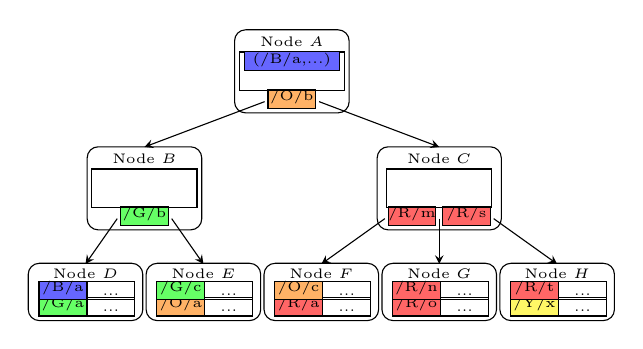
\begin{tikzpicture}[xscale=0.95, yscale=0.95]
        \node[anchor=south, rectangle, rounded corners, minimum height=.06\textwidth, minimum width=.12\textwidth, draw=black] at (0, 0) {};
        \node[anchor=south, font=\tiny] at (0, .036\textwidth) {Node $F$};
        \node[anchor=south, rectangle, minimum height=.015\textwidth, minimum width=.05\textwidth, draw=black, fill={red!60}] at (-.025\textwidth, .005\textwidth) {};
        \node[anchor=south, font=\tiny] at (-.025\textwidth, 0) {/R/a};
        \node[anchor=south, rectangle, minimum height=.015\textwidth, minimum width=.05\textwidth, draw=black] at (.028\textwidth, .005\textwidth) {};
        \node[anchor=south, font=\tiny] at (.028\textwidth, 0) {...};
        \node[anchor=south, rectangle, minimum height=.015\textwidth, minimum width=.05\textwidth, draw=black, fill={orange!60}] at (-.025\textwidth, .023\textwidth) {};
        \node[anchor=south, font=\tiny] at (-.025\textwidth, .018\textwidth) {/O/c};
        \node[anchor=south, rectangle, minimum height=.015\textwidth, minimum width=.05\textwidth, draw=black] at (.028\textwidth, .023\textwidth) {};
        \node[anchor=south, font=\tiny] at (.028\textwidth, .018\textwidth) {...};

        \node[anchor=south, rectangle, rounded corners, minimum height=.06\textwidth, minimum width=.12\textwidth, draw=black] at (.13\textwidth, 0) {};
        \node[anchor=south, font=\tiny] at (.13\textwidth, .036\textwidth) {Node $G$};
        \node[anchor=south, rectangle, minimum height=.015\textwidth, minimum width=.05\textwidth, draw=black, fill={red!60}] at (.105\textwidth, .005\textwidth) {};
        \node[anchor=south, font=\tiny] at (.105\textwidth, 0) {/R/o};
        \node[anchor=south, rectangle, minimum height=.015\textwidth, minimum width=.05\textwidth, draw=black] at (.158\textwidth, .005\textwidth) {};
        \node[anchor=south, font=\tiny] at (.158\textwidth, 0) {...};
        \node[anchor=south, rectangle, minimum height=.015\textwidth, minimum width=.05\textwidth, draw=black, fill={red!60}] at (.105\textwidth, .023\textwidth) {};
        \node[anchor=south, font=\tiny] at (.105\textwidth, .018\textwidth) {/R/n};
        \node[anchor=south, rectangle, minimum height=.015\textwidth, minimum width=.05\textwidth, draw=black] at (.158\textwidth, .023\textwidth) {};
        \node[anchor=south, font=\tiny] at (.158\textwidth, .018\textwidth) {...};

        \node[anchor=south, rectangle, rounded corners, minimum height=.06\textwidth, minimum width=.12\textwidth, draw=black] at (.26\textwidth, 0) {};
        \node[anchor=south, font=\tiny] at (.26\textwidth, .036\textwidth) {Node $H$};
        \node[anchor=south, rectangle, minimum height=.015\textwidth, minimum width=.05\textwidth, draw=black, fill={yellow!60}] at (.235\textwidth, .005\textwidth) {};
        \node[anchor=south, font=\tiny] at (.235\textwidth, 0) {/Y/x};
        \node[anchor=south, rectangle, minimum height=.015\textwidth, minimum width=.05\textwidth, draw=black] at (.288\textwidth, .005\textwidth) {};
        \node[anchor=south, font=\tiny] at (.288\textwidth, 0) {...};
        \node[anchor=south, rectangle, minimum height=.015\textwidth, minimum width=.05\textwidth, draw=black, fill={red!60}] at (.235\textwidth, .023\textwidth) {};
        \node[anchor=south, font=\tiny] at (.235\textwidth, .018\textwidth) {/R/t};
        \node[anchor=south, rectangle, minimum height=.015\textwidth, minimum width=.05\textwidth, draw=black] at (.288\textwidth, .023\textwidth) {};
        \node[anchor=south, font=\tiny] at (.288\textwidth, .018\textwidth) {...};

        \node[anchor=south, rectangle, rounded corners, minimum height=.06\textwidth, minimum width=.12\textwidth, draw=black] at (-.13\textwidth, 0) {};
        \node[anchor=south, font=\tiny] at (-.13\textwidth, .036\textwidth) {Node $E$};
        \node[anchor=south, rectangle, minimum height=.015\textwidth, minimum width=.05\textwidth, draw=black, fill={orange!60}] at (-.155\textwidth, .005\textwidth) {};
        \node[anchor=south, font=\tiny] at (-.155\textwidth, 0) {/O/a};
        \node[anchor=south, rectangle, minimum height=.015\textwidth, minimum width=.05\textwidth, draw=black] at (-.102\textwidth, .005\textwidth) {};
        \node[anchor=south, font=\tiny] at (-.102\textwidth, 0) {...};
        \node[anchor=south, rectangle, minimum height=.015\textwidth, minimum width=.05\textwidth, draw=black, fill={green!60}] at (-.155\textwidth, .023\textwidth) {};
        \node[anchor=south, font=\tiny] at (-.155\textwidth, .018\textwidth) {/G/c};
        \node[anchor=south, rectangle, minimum height=.015\textwidth, minimum width=.05\textwidth, draw=black] at (-.102\textwidth, .023\textwidth) {};
        \node[anchor=south, font=\tiny] at (-.102\textwidth, .018\textwidth) {...};

        \node[anchor=south, rectangle, rounded corners, minimum height=.06\textwidth, minimum width=.12\textwidth, draw=black] at (-.26\textwidth, 0) {};
        \node[anchor=south, font=\tiny] at (-.26\textwidth, .036\textwidth) {Node $D$};
        \node[anchor=south, rectangle, minimum height=.015\textwidth, minimum width=.05\textwidth, draw=black, fill={green!60}] at (-.285\textwidth, .005\textwidth) {};
        \node[anchor=south, font=\tiny] at (-.285\textwidth, 0) {/G/a};
        \node[anchor=south, rectangle, minimum height=.015\textwidth, minimum width=.05\textwidth, draw=black] at (-.232\textwidth, .005\textwidth) {};
        \node[anchor=south, font=\tiny] at (-.232\textwidth, 0) {...};
        \node[anchor=south, rectangle, minimum height=.015\textwidth, minimum width=.05\textwidth, draw=black, fill={blue!60}] at (-.285\textwidth, .023\textwidth) {};
        \node[anchor=south, font=\tiny] at (-.285\textwidth, .018\textwidth) {/B/a};
        \node[anchor=south, rectangle, minimum height=.015\textwidth, minimum width=.05\textwidth, draw=black] at (-.232\textwidth, .023\textwidth) {};
        \node[anchor=south, font=\tiny] at (-.232\textwidth, .018\textwidth) {...};

        \node[anchor=south, rectangle, rounded corners, minimum height=.087\textwidth, minimum width=.12\textwidth, draw=black] at (-.195\textwidth, .1\textwidth) {};
        \node[anchor=south, font=\tiny] at (-.195\textwidth, .163\textwidth) {Node $B$};
        \node[anchor=south, rectangle, minimum height=.015\textwidth, minimum width=.05\textwidth, draw=black, fill={green!60}] at (-.195\textwidth, .105\textwidth) {};
        \node[anchor=south, font=\tiny] at (-.195\textwidth, .1\textwidth) {/G/b};
        \node[anchor=south, rectangle, minimum height=.04\textwidth, minimum width=.11\textwidth, draw=black] at (-.195\textwidth, .125\textwidth) {};

        \node[anchor=south, rectangle, rounded corners, minimum height=.087\textwidth, minimum width=.13\textwidth, draw=black] at (.13\textwidth, .1\textwidth) {};
        \node[anchor=south, font=\tiny] at (.13\textwidth, .163\textwidth) {Node $C$};
        \node[anchor=south, rectangle, minimum height=.015\textwidth, minimum width=.05\textwidth, draw=black, fill={red!60}] at (.1\textwidth, .105\textwidth) {};
        \node[anchor=south, font=\tiny] at (.1\textwidth, .1\textwidth) {/R/m};
        \node[anchor=south, rectangle, minimum height=.015\textwidth, minimum width=.05\textwidth, draw=black, fill={red!60}] at (.16\textwidth, .105\textwidth) {};
        \node[anchor=south, font=\tiny] at (.16\textwidth, .1\textwidth) {/R/s};
        \node[anchor=south, rectangle, minimum height=.04\textwidth, minimum width=.11\textwidth, draw=black] at (.13\textwidth, .125\textwidth) {};

        \node[anchor=south, rectangle, rounded corners, minimum height=.087\textwidth, minimum width=.12\textwidth, draw=black] at (-.0325\textwidth, .229\textwidth) {};
        \node[anchor=south, font=\tiny] at (-.0325\textwidth, .292\textwidth) {Node $A$};
        \node[anchor=south, rectangle, minimum height=.015\textwidth, minimum width=.05\textwidth, draw=black, fill={orange!60}] at (-.0325\textwidth, .234\textwidth) {};
        \node[anchor=south, font=\tiny] at (-.0325\textwidth, .229\textwidth) {/O/b};
        \node[anchor=south, rectangle, minimum height=.04\textwidth, minimum width=.11\textwidth, draw=black] at (-.0325\textwidth, .254\textwidth) {};
        \node[anchor=south, rectangle, minimum height=.015\textwidth, minimum width=.1\textwidth, draw=black, fill={blue!60}] at (-.0325\textwidth, .276\textwidth) {};
        \node[anchor=south, font=\tiny] at  (-.0325\textwidth, .27\textwidth) {\upsertm(/B/a,...)};

        \draw[->, >=stealth] (-.225\textwidth, .113\textwidth) -- (-.26\textwidth, .063\textwidth);
        \draw[->, >=stealth] (-.165\textwidth, .113\textwidth) -- (-.13\textwidth, .063\textwidth);
        \draw[->, >=stealth] (.13\textwidth, .113\textwidth) -- (.13\textwidth, .063\textwidth);
        \draw[->, >=stealth] (.19\textwidth, .113\textwidth) -- (.26\textwidth, .063\textwidth);
        \draw[->, >=stealth] (.07\textwidth, .113\textwidth) -- (0, .063\textwidth);
        \draw[->, >=stealth] (-.0625\textwidth, .242\textwidth) -- (-.195\textwidth, .192\textwidth);
        \draw[->, >=stealth] (-.0025\textwidth, .242\textwidth) -- (.13\textwidth, .192\textwidth);
    \end{tikzpicture}
    \caption[An example of an upsert in a \bet]{\label{fig:upsert}
        An upsert message stores the description of modification on the old
        value associated with the key.}
\end{figure}

Figure~\ref{fig:upsert} shows an example of an \upsertm message in the \bet.
In the example, the application wants to update the value associated with
the key ``/B/a''.
Instead of querying the \bet for the old value and then inserting the new value,
the application calls the upsert operation that injects an \upsertm message into
the root node, Node $A$.
Assume the old value associated with the key ``/B/a'' in Node $D$ is $v$,
the delta in the \upsertm message is $\Delta$,
and the user-specified function is $f$.
The \upsertm message essentially updates the value associated with the key
``/B/a'' to $f(v,\Delta)$.
Queries for the key ``/B/a'' need to calculate $f(v,\Delta)$ on the fly.
And the \upsertm message will update the value associated with the key ``/B/a''
to $f(v,\Delta)$ when the \bet flushes the message to Node $D$.

\section{Full-path-indexed \betrfs}
\label{sec:bg:fpi}

\begin{figure}[t]
    \centering
    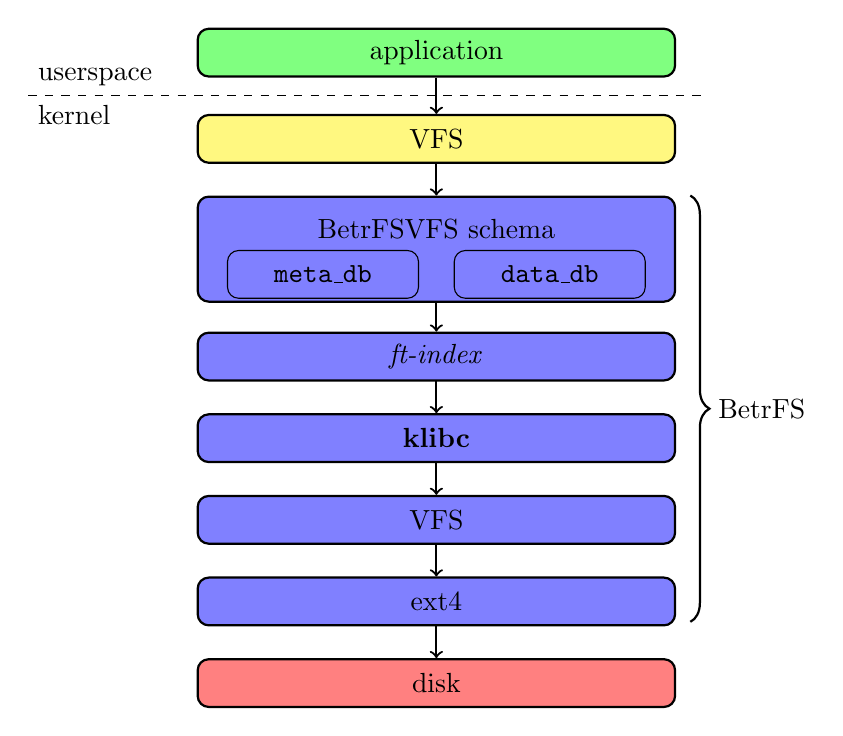
\begin{tikzpicture}[yscale=0.95, xscale=0.95]
    \draw[thick, ->] (0, .04\textwidth) -- (0, 0) node [anchor=north, rectangle, rounded corners, text centered, minimum height=.05\textwidth, minimum width=.5\textwidth, draw=black, fill=red!50] {disk};
    \draw[thick, ->] (0, .13\textwidth) -- (0, .09\textwidth) node [anchor=north, rectangle, rounded corners, text centered, minimum height=.05\textwidth, minimum width=.5\textwidth, draw=black, fill=blue!50] {ext4};
    \draw[thick, ->] (0, .22\textwidth) -- (0, .18\textwidth) node [anchor=north, rectangle, rounded corners, text centered, minimum height=.05\textwidth, minimum width=.5\textwidth, draw=black, fill=blue!50] {VFS};
    \draw[thick, ->] (0, .31\textwidth) -- (0, .27\textwidth) node [anchor=north, rectangle, rounded corners, text centered, minimum height=.05\textwidth, minimum width=.5\textwidth, draw=black, fill=blue!50] {\klibc};
    \draw[thick, ->] (0, .4\textwidth) -- (0, .36\textwidth) node [anchor=north, rectangle, rounded corners, text centered, minimum height=.05\textwidth, minimum width=.5\textwidth, draw=black, fill=blue!50] {\fti};
    \draw[thick, ->] (0, .55\textwidth) -- (0, .51\textwidth) node [anchor=north, rectangle, rounded corners, text centered, minimum height=.11\textwidth, minimum width=.5\textwidth, draw=black, fill=blue!50] {};
    \node [anchor=north, rectangle, rounded corners, text centered, minimum height=.05\textwidth, minimum width=.2\textwidth, draw=black, fill=blue!50] at (.125\textwidth, .45\textwidth) {\ddb};
    \node [anchor=north, rectangle, rounded corners, text centered, minimum height=.05\textwidth, minimum width=.2\textwidth, draw=black, fill=blue!50] at (-.125\textwidth, .45\textwidth) {\mdb};
    \node [anchor=north, text centered, minimum height=.05\textwidth] at (0, .50\textwidth) {\betrfs VFS schema};
    \draw[thick, ->] (0, .64\textwidth) -- (0, .60\textwidth) node [anchor=north, rectangle, rounded corners, text centered, minimum height=.05\textwidth, minimum width=.5\textwidth, draw=black, fill=yellow!50] {VFS};
    \node[anchor=south, rectangle, rounded corners, text centered, minimum height=.05\textwidth, minimum width=.5\textwidth, draw=black, thick, fill=green!50] at (0, .64\textwidth) {application};
    \draw[dashed] (-.45\textwidth, .62\textwidth) -- (.3\textwidth, .62\textwidth);
    \node[anchor=south west] at (-.45\textwidth, .62\textwidth) {userspace};
    \node[anchor=north west] at (-.45\textwidth, .62\textwidth) {kernel};
    \draw[decorate, decoration={brace,amplitude=.02\textwidth,mirror}, thick] (.28\textwidth, .04\textwidth) -- (.28\textwidth, .51\textwidth);
    \node[anchor=west,text centered] at (.3\textwidth, .275\textwidth) {\betrfs};
    \end{tikzpicture}
    \caption[The \betrfs architecture]{\label{fig:betrfs}
        The \betrfs architecture.}
\end{figure}

\betrfs~\citep{betrfs1,betrfs1tos} is a Linux in-kernel, full-path-indexed,
write-optimized file system built upon \fti~\citep{fti},
a key/value store that implements \bets and
exposes a key/value interface similar to Berkeley DB.

Figure~\ref{fig:betrfs} shows the \betrfs architecture.
In Linux, applications interact with file systems through system calls,
which invoke the corresponding VFS (Virtual File System) functions.
The VFS function then calls the particular function implemented by
the underlying file system.
\betrfs implements file systems operations by translating them into key/value
store operations in \fti.
\betrfs interacts with \fti through point operations, such as \texttt{put},
\texttt{get} and \texttt{del}, as well as range queries with cursors
(\texttt{c\_get} with DB\_SET\_RANGE and DB\_NEXT).
\betrfs also uses the transaction interface of \fti to execute multiple
operations atomically in one transaction.
A redo log and periodic checkpoints (every 60 seconds) in \fti ensure that
changes are made persistent on the disk.

\Fti cannot be integrated into a Linux kernel module easily because
it is a userspace library that assumes libc functions and system calls.
To address this issue, we built a shim layer called \klibc in \betrfs.
\Klibc implements all functions \fti requires.
For example, \fti requires a underlying file system to perform file operations.
To this end, \klibc privately mounts an ext4 file system and calls the
corresponding VFS functions when \fti invokes file system operations.
Through a shim layer, \betrfs can incorporate \fti into the kernel module
without modifying code in \fti.

\betrfs uses two key/value indexes to store metadata and data in the file
system.
One index, \mdb, stores metadata, mapping full-paths to \texttt{struct stat}
structures.
The other index, \ddb, stores data, mapping (full-path and block number) to
4KiB blocks.
When the file system function needs metadata, \betrfs queries
the \mdb with the full-path key and constructs the corresponding inode
from the \texttt{struct stat}.
Likewise, when a dirty inode needs to be written, the \texttt{struct stat} is
assembled from the inode and written to the \mdb with the
full-path key.
Blocks of a file are fetched and written by the full-path and the indexes of
blocks.
Although other block granularity is possible (we tried 512B for the preliminary
implementation of \betrfs), 4KiB is the natural block size
because it is the same as the page size in the Linux page cache.

\betrfs can write to a block without fetching the old block to memory, avoiding
expensive read-before-write described in Section~\ref{sec:bg:bet}.
Conventional file systems must read the old block from the disk to the page
cache before writing to that block (a complete overwrite can be done without
fetching the old block, but it is not implemented in any file system).
However, \bets have asymmetric read and write costs, so read-before-write should
be avoided.
In \betrfs, if the corresponding block is not in memory, an upsert message,
which describes the offset, length and content of this write, is injected into
the root node of the \bet.
When this upsert message is flushed to the leaf node, the change is applied to
the old block.

Write-optimized \bets make random writes much faster in \betrfs than
conventional file systems.
Unlike other file systems,
which performs each random write at a random locality on the disk,
\betrfs usually resolves a random write by injecting a message into the root
node of the \bet
and flushes messages in batches.
Because random I/Os are much slower than sequential I/Os on disks,
\betrfs have much better random write performance.

Also, full-path indexing in \betrfs ensures locality even with file system
aging~\citep{betrfs3}.
After \betrfs fetches one block of a file from the disk, all nodes along the
root-to-leaf path are present in memory.
And with full-path indexing, all keys under one directory are contiguous in the
key space, which means a subsequent fetch of some other block in the same file or
another file under than same directory is likely to be resolved in memory,
which significantly increases performance and I/O efficiency.

The first implementation of \betrfs (\betrfsOne) shows great random write
performance.
Recursive greps run 3.77x faster than in the best standard file system.
File creation runs 12.54x faster.
Small, random writes to a file run 68.24x faster~\citep{betrfs1tos}.

However, namespace operations have predictably miserable performance in
\betrfsOne.
Deleting and renaming a Linux source directory take 46.14 and 21.17 seconds,
respectively, because the file system has to call one or more key/value store
operations for each key.

Later, we fixed the delete problem with range-delete messages~\citep{betrfs2,betrfs2tos}.
A range-delete message invalidates all key/value pairs within its key range.
When flushing a range-delete message, the \bet injects the message into all
children whose key ranges overlap with the range-delete message.
Upon reaching a leaf node, the range-delete message deletes all key/value pairs
within its key range.

However, the rename problem remains difficult in full-path-indexed \betrfs
because a rename needs to update all affected keys in the \bets,
an operation that is uncommon in key/value stores.

\section{Relative-path-indexed \betrfs}
\label{sec:bg:rpi}

\begin{figure}[t]
    \begin{subfigure}[t]{.5\textwidth}
        \centering
        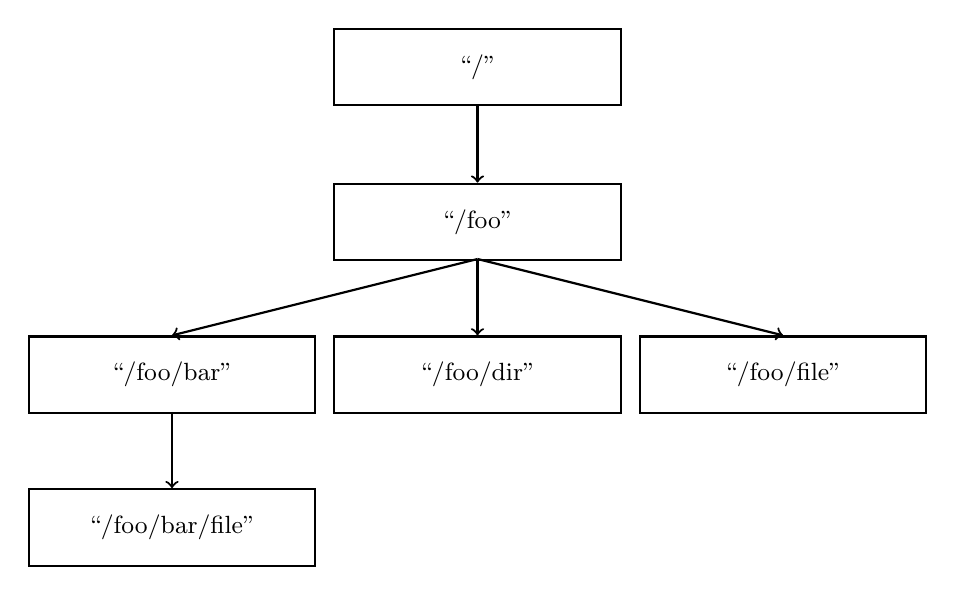
\begin{tikzpicture}{xscale=0.95,yscale=0.95}
            \draw[thick, ->] (0, .08\textwidth) -- (0, 0) node [anchor=north, rectangle, text centered, minimum height=.08\textwidth, minimum width=.3\textwidth, draw=black, font=\small] {``/foo/bar/file''};
            \draw[thick, ->] (.32\textwidth, .24\textwidth) -- (0, .16\textwidth) node [anchor=north, rectangle, text centered, minimum height=.08\textwidth, minimum width=.3\textwidth, draw=black, font=\small] {``/foo/bar''};
            \draw[thick, ->] (.32\textwidth, .24\textwidth) -- (.32\textwidth, .16\textwidth) node [anchor=north, rectangle, text centered, minimum height=.08\textwidth, minimum width=.3\textwidth, draw=black, font=\small] {``/foo/dir''};
            \draw[thick, ->] (.32\textwidth, .24\textwidth) -- (.64\textwidth, .16\textwidth) node [anchor=north, rectangle, text centered, minimum height=.08\textwidth, minimum width=.3\textwidth, draw=black, font=\small] {``/foo/file''};
            \draw[thick, ->] (.32\textwidth, .4\textwidth) -- (.32\textwidth, .32\textwidth) node [anchor=north, rectangle, text centered, minimum height=.08\textwidth, minimum width=.3\textwidth, draw=black, font=\small] {``/foo''};
            \node [anchor=south, rectangle, text centered, minimum height=.08\textwidth, minimum width=.3\textwidth, draw=black, thick, font=\small] at (.32\textwidth, .4\textwidth) {``/''};
        \end{tikzpicture}
        \caption{\label{subfig:FPI} Full-path indexing only keeps full-paths.}
    \end{subfigure}
    \begin{subfigure}[t]{.5\textwidth}
        \centering
        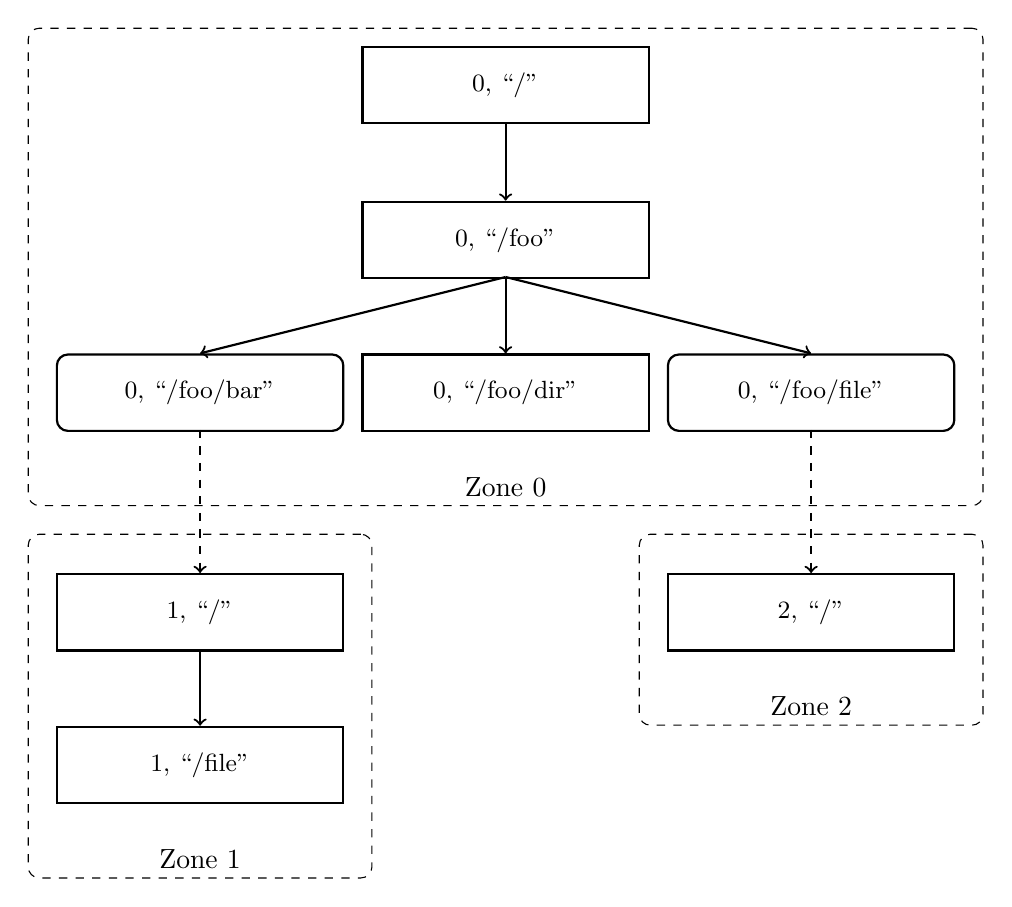
\begin{tikzpicture}{xscale=0.95,yscale=0.95}
            \node [anchor=south, rectangle, rounded corners, minimum height=.50\textwidth, minimum width=\textwidth, draw=black, dashed] at (.32\textwidth, 0) {};
            \node [anchor=south] at (.32\textwidth, 0) {Zone 0};
            \draw[thick, ->] (.32\textwidth, .24\textwidth) -- (0, .16\textwidth) node [anchor=north, rectangle, rounded corners, text centered, minimum height=.08\textwidth, minimum width=.3\textwidth, draw=black, font=\small] {0, ``/foo/bar''};
            \draw[thick, ->] (.32\textwidth, .24\textwidth) -- (.32\textwidth, .16\textwidth) node [anchor=north, rectangle, text centered, minimum height=.08\textwidth, minimum width=.3\textwidth, draw=black, font=\small] {0, ``/foo/dir''};
            \draw[thick, ->] (.32\textwidth, .24\textwidth) -- (.64\textwidth, .16\textwidth) node [anchor=north, rectangle, rounded corners, text centered, minimum height=.08\textwidth, minimum width=.3\textwidth, draw=black, font=\small] {0, ``/foo/file''};
            \draw[thick, ->] (.32\textwidth, .4\textwidth) -- (.32\textwidth, .32\textwidth) node [anchor=north, rectangle, text centered, minimum height=.08\textwidth, minimum width=.3\textwidth, draw=black, font=\small] {0, ``/foo''};
            \node [anchor=south, rectangle, text centered, minimum height=.08\textwidth, minimum width=.3\textwidth, draw=black, thick, font=\small] at (.32\textwidth, .4\textwidth) {0, ``/''};
            \node [anchor=south, rectangle, rounded corners, minimum height=.36\textwidth, minimum width=.36\textwidth, draw=black, dashed] at (0, -.39\textwidth) {};
            \node [anchor=south] at (0, -.39\textwidth) {Zone 1};
            \node [anchor=north, rectangle, text centered, minimum height=.08\textwidth, minimum width=.3\textwidth, draw=black, thick, font=\small] at (0, -.07\textwidth) {1, ``/''};
            \draw[thick, ->] (0, -.15\textwidth) -- (0, -.23\textwidth) node [anchor=north, rectangle, text centered, minimum height=.08\textwidth, minimum width=.3\textwidth, draw=black, font=\small] {1, ``/file''};
            \node [anchor=south, rectangle, rounded corners, minimum height=.2\textwidth, minimum width=.36\textwidth, draw=black, dashed] at (.64\textwidth, -.23\textwidth) {};
            \node [anchor=south] at (.64\textwidth, -.23\textwidth) {Zone 2};
            \node [anchor=north, rectangle, text centered, minimum height=.08\textwidth, minimum width=.3\textwidth, draw=black, thick, font=\small] at (.64\textwidth, -.07\textwidth) {2, ``/''};
            \draw[thick, dashed, ->] (0, .08\textwidth) -- (0, -.07\textwidth);
            \draw[thick, dashed, ->] (.64\textwidth, .08\textwidth) -- (.64\textwidth, -.07\textwidth);
        \end{tikzpicture}
        \caption{\label{subfig:RPI} Relative-path indexing splits the directory tree into zones and
            uses indirection between zones.}
    \end{subfigure}
    \caption[Full-path indexing and relative-path indexing]{\label{fig:FPIRPI}
        The same directory tree under full-path indexing and relative-path indexing.}
\end{figure}

Relative-path-indexed \betrfs~\citep{betrfs2,betrfs2tos} backed away from
full-path indexing and introduced relative-path indexing,
which is also called zoning.
Relative-path indexing partitions the directory hierarchy into zones.
Each zone has a zone ID (the root zone always has zone ID 0), which is analogous
to an inode number, and a single root file or directory.
All file or directory in a zone is indexed relative to the zone root.
If the file or directory is the root of another zone, the entry contains the
zone ID to redirect queries.
With the introduction of zoning, each key in \betrfs contains two parts,
a zone ID and the relative path to the zone root.

Figure~\ref{fig:FPIRPI} shows an example of the same directory tree under
full-path indexing and relative-path indexing.
In Figure~\ref{subfig:RPI}, relative-path indexing partitions the directory
into three zones.
Zone 0 is the root zone, Zone 1 is rooted at a directory ``/foo/bar'' and
Zone 2 is rooted at a file ``/foo/file''.
When querying the key/value store for file ``/foo/file'' with key
(0, ``/foo/file''), the file system gets a special value that
indicates the entry is the root of Zone 2.
Subsequently, the file system queries the key/value store with key (2, ``/'')
and gets the correct value.
Similarly, the file system notices the key for directory ``/foo/bar'' is
(3, ``/'').
Therefore, when querying for file ``/foo/bar/file'', it uses key (3, ``/file'').

Relative-path indexing tries to balance locality and rename performance through
a target zone size.
On one hand, full-path indexing is still maintained within a zone,
so larger zone size gives better locality.
On the other hand, smaller zone size imposes a lower bound on rename cost,
because no rename needs to mutate more key/value pairs than the zone size.
Relative-path-indexing with an infinite zone size is equivalent to
full-path-indexing, while relative-path-indexing with a zero zone size is the
same as indexing with inode numbers.

Relative-path indexing keeps zones within the target zone size by zone splits
and merges.
In particular, for each file or directory, \betrfs keeps a counter in its inode
to indicate how many key/value pairs will be affected if the file or directory
is renamed.
When the counter of a directory or file becomes too big,
relative-path indexing moves it to its own zone with a zone split,
updating all affected keys with the new zone ID and relative-paths.
When the counter of a zone root becomes too small (1/4 of the maximum
size), relative-path indexing merges it to the parent zone.

\begin{figure}[t]
    \centering
    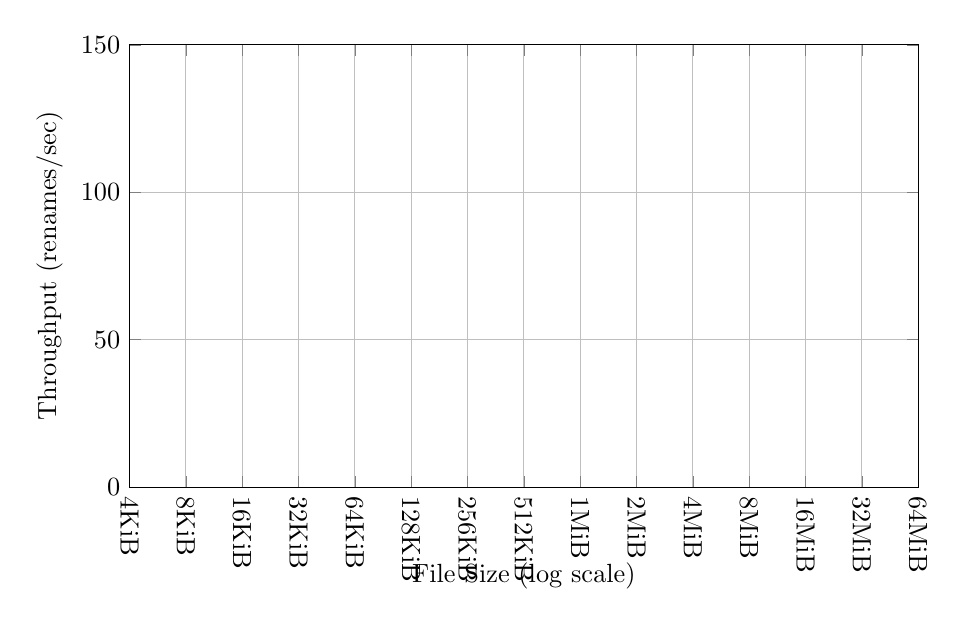
\begin{tikzpicture}[yscale=0.95, xscale=0.95]
        \begin{axis}[
                xlabel={File Size (log scale)},
                x label style={at={(axis description cs:0.5,-0.15)},anchor=north},
                ylabel={Throughput (renames/sec)},
                xmin=12,
                xmax=26,
                xtick={12,13,14,15,16,17,18,19,20,21,22,23,24,25,26},
                xticklabels={4KiB,8KiB,16KiB,32KiB,64KiB,128KiB,256KiB,512KiB,1MiB,2MiB,4MiB,8MiB,16MiB,32MiB,64MiB},
                xticklabel style={rotate=270, anchor=west},
                ymin=0,
                ymax=150,
                grid=major,
                scaled x ticks=false,
                scaled y ticks=false,
                legend columns=4,
                legend cell align=left,
                height=.618\linewidth,
                width=\linewidth,
            ]
            \addFileRenamePlot{ext4};
            \addFileRenamePlot{btrfs};
            \addFileRenamePlot{xfs};
            \addFileRenamePlot{zfs};
            \addFileRenamePlot{nilfs2};
            \addFileRenamePlot{betrfs3};
            \addFileRenamePlot{betrfs3-max};
        \end{axis}
    \end{tikzpicture}
    \caption[The performance of file renames in relative-path-indexed file systems]{\label{fig:file_rename_rpi}
        Throughput of renaming a file of different sizes (higher is better).
        The performance of relative-path-indexed \betrfsThree doesn't
        degrade when the file being renamed becomes larger.}
\end{figure}

The implementation of relative-path-indexed \betrfs, \betrfsTwo, adopts a
512KiB default zone size.
This default zone size is small enough that renames on \betrfsTwo are almost
as fast as on inode-based file systems.
At the same time, the default zone size is large enough that directory
traversals are almost as fast as \betrfsOne.

Figure~\ref{fig:file_rename_rpi} shows the results of running the file rename
benchmark on \betrfsThree (\betrfsThree is \betrfsTwo with some bug fixes).
The benchmark renames a file of different sizes 100 times, each followed by a
\texttt{fsync} of the parent directory.
We run the benchmark on \betrfsThree twice,
one on \betrfsThree (with the default zone size),
the other on full-path-indexed \betrfsThree,
that is, \betrfsThree with an infinite zone size.
As shown in the graph, before reaching the target zone size, 512KiB,
the performance of relative-path-indexed \betrfsThree is similar to
full-path-indexed \betrfsThree.
However, when the file size reaches the target zone size, the file forms its
own zone and file renames become pointer swings.
Therefore, after the target zone size,
the performance of file renames in relative-path-indexed \betrfsThree
doesn't degrade when the file size becomes larger.

\begin{table}[t]
    \centering
    \begin{tabular}{l|.@{${}\pm{}$}.}
    \hline
    File system & \multicolumn{2}{c}{grep (sec)}  \\
    \hline
    \hline
    \pgfkeysvalueof{/fs-names/ext4}        &  37.795 &  1.145 \\
    \pgfkeysvalueof{/fs-names/btrfs}       &   9.265 &  0.139 \\
    \pgfkeysvalueof{/fs-names/xfs}         &  48.130 &  0.206 \\
    \pgfkeysvalueof{/fs-names/zfs}         & 463.184 & 33.878 \\
    \pgfkeysvalueof{/fs-names/nilfs2}      &   8.318 &  0.107 \\
    \pgfkeysvalueof{/fs-names/betrfs3}     &   5.070 &  0.078 \\
    \pgfkeysvalueof{/fs-names/betrfs3-max} &   4.022 &  0.055 \\
    \hline
    \end{tabular}
    \caption[The performnace of directory traversals in relative-path-indexed file systems]{\label{tab:dir_ops_rpi}
        Time to perform recursive grep of the Linux source directory (lower is better).
        The performance of relative-path-indexed \betrfsThree is still better than
        conventional file systems.}
\end{table}

Table~\ref{tab:dir_ops_rpi} shows the performance of directory traversals on
different file systems.
The benchmark measures the time to \texttt{grep} the  Linux 3.11.10 source
directory.
Relative-path-indexed \betrfsThree is slightly slower than full-path-indexed
\betrfsThree, but still faster than other file systems.

\begin{figure}[t]
    \centering
    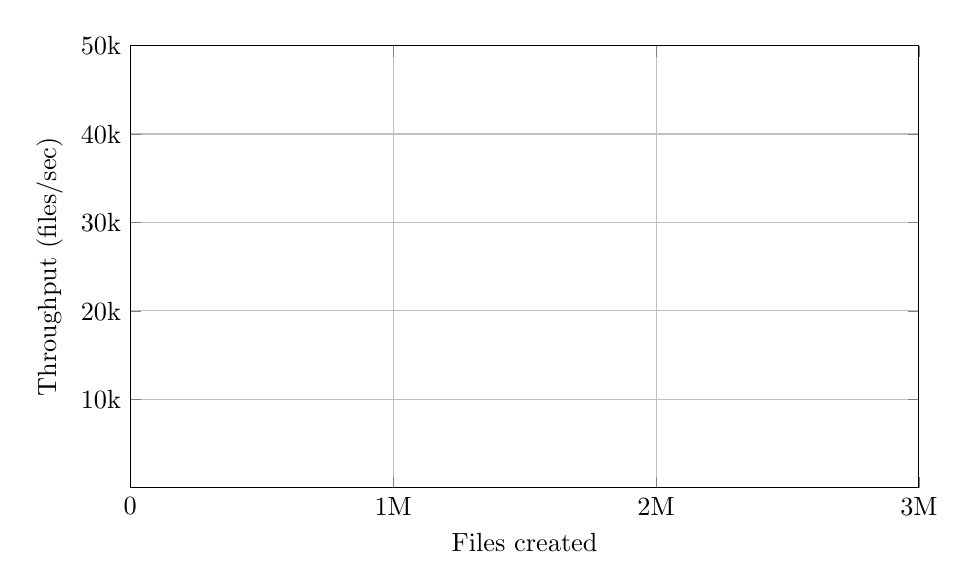
\begin{tikzpicture}[yscale=0.95,xscale=0.95]
        \begin{axis}[
            xlabel={Files created},
            ylabel={Throughput (files/sec)},
            xmin=0,
            xmax=3000000,
            ymin=10,
            ymax=50000,
            mark repeat=10,
            xtick={0,1000000,2000000,3000000},
            xticklabels={0,1M,2M,3M},
            ytick={10000,20000,30000,40000,50000},
            yticklabels={10k,20k,30k,40k,50k},
            grid=major,
            scaled x ticks=false,
            scaled y ticks=false,
            legend cell align=left,
            transpose legend,
            height=.618\linewidth,
            width=\linewidth,
        ]
        \addTokubenchPlot{betrfs3};
        \addTokubenchPlot{betrfs3-max};
        \end{axis}
    \end{tikzpicture}
    \caption[Zone maintainance cost in TokuBench benchmark]{
        Cumulative file creation throughput during the Tokubench benchmark (higher is better).
        Compared to full-path-indexed \betrfsThree,
        relative-path-indexed \betrfsThree has a sudden
        performance drop because of zone splits.}
    \label{fig:tokuzone}
\end{figure}

However, relative-path indexing imposes zone maintenance costs on other file
system operations.
When a file system operation happens to trigger a zone split or merge,
in addition to the costs of the operation itself,
relative-path indexing charges the zone split or merge to that operations.
For instance, Figure~\ref{fig:tokuzone} shows the results of running Tokubench,
which creates 3 million small files in a balanced tree structure,
on \betrfsThree.
On the graph, two-thirds of the way through the TokuBench benchmark,
\betrfsThree with the default zone size shows a sudden,
precipitous drop in cumulative throughput for small file creation,
because the file system performs a huge amount of zone splits.
At that moment, all benchmarking directories are one file less than the target
zone size.
Therefore, creating one file in a directory results in a zone split,
updating all key/value pairs under the directory.
On the contrary, \betrfsThree with an infinite zone size
has a smooth curve throughout the benchmark
because no zone split happens with a infinite zone size.

Furthermore, relative-path indexing has bad worst-case performance.
It is possible to construct arrangements of nested directories that will each
reside in their own zone.
Reading a file in the deepest directory will require reading one zone per
directory (each with its own I/O),
essentially making the file system inode-based.
Such a pathological worst case is not possible with full-path indexing in a
\bet, and an important design goal for \betrfs is keeping a reasonable bound on
the worst cases.

Finally, relative-path indexing breaks the clean mapping of directory subtrees
onto contiguous ranges of the key space,
preventing us from using range-messages to implement bulk operations on entire
directory.
For example, with full-path indexing, we can use range-delete messages not
only to delete files, but an entire directory.
We could also use range messages to perform a variety of other operations on
the whole directory, such as recursive \texttt{chmod}, \texttt{chown} and
timestamp updates.
And, as we will eventually see with the range-clone operations, we can clone the
whole directory with one operation.

\section{Implementation}
\label{sec:bg:impl}

\section{Conclusion}

\betrfs is a general file system designed for all operations, with a particular
focus on random writes and locality.
The underlying data structure, \bets, performs random writes much faster than
\btrees by cascading writes in batches.
The full-path indexing schema of \betrfsOne ensures good locality.
However, the preliminary implementation of namespace operations in \betrfsOne
is slow because they need to iterate all affected keys.
The relative-path indexing schema of \betrfsTwo enables fast renames by bounding
the maximum number of affected in a rename.
However, it imposes zone maintenance costs on other file system operations.
Also, it breaks the full-path indexing, preventing us from implementing other
efficient namespace operations that are difficult on other file systems.



\chapter{Renaming}
\label{chap:rename}

Renaming


\input{cloning}

\chapter{Evaluation}
\label{chap:eval}

This chapter evaluates the performance of \betrfs with
range-rename (\betrfsFour) and \betrfs with range-clone (\betrfsFive).
The evaluation includes the following four aspects:
(1) performance of single file-system operations;
(2) performance of widely used applications;
(3) performance of renames;
(4) performance of clones.

\paragraph{Experimental Setup.}

All experimental results were collected on
a Dell Optiplex 790 with a 4-core 3.40 GHz Intel Core i7-2600 CPU,
4GB RAM,
and a 500 GB, 7200 SATA disk with a 4096-byte block size(Seagate Barracuda ST500DM002).
The system runs 64-bit Ubuntu server 14.04.05 on a USB stick to prevent
interference form the root file system.
\betrfsFour runs on a modified Linux-3.11.10 kernel that enlarges the size of the kernel stack,
while \betrfsFive and all other file systems run on Linux-4.9.142 kernel.
The evaluation uses ZFS 0.6.5.11 from \url{zfsonlinx.org} and
ext4, Btrfs, XFS and NILFS2 as parts of the Linux kernel.
Each experiment runs a minimum of 5 times and reports the median number.
Error bars indicate minimum and maximum numbers over all runs.
Similarly, error $\pm$ terms bound minimum and maximum numbers over all runs.
Unless noted, all benchmarks are cold-cache tests.

\section{Microbenchmarks}

\paragraph{Sequential writes and reads.}

We measure the throughput of sequentially writing and reading a file.
This benchmark first writes a 10-GiB file, 64 blocks at a time, with a
\texttt{fsync} to flush the file to disk.
Then, after cleaning the kernel page cache, the kernel reads the file from disk.

\newcommand{\addSeqPlot}[1]{
    \addplot[
        discard if not={fs}{#1},
        fill=\pgfkeysvalueof{/fs-colors/#1},
        nodes near coords=\pgfkeysvalueof{/fs-names/#1},
    ]
    plot[
        error bars/.cd,
        y dir=both, y explicit,
    ]
    table[
        x=op,
        y=median,
        y error plus expr=\thisrow{max}-\thisrow{median},
        y error minus expr=\thisrow{median}-\thisrow{min},
    ]
    {./data/seq_io.csv};
}

\begin{figure}[t]
    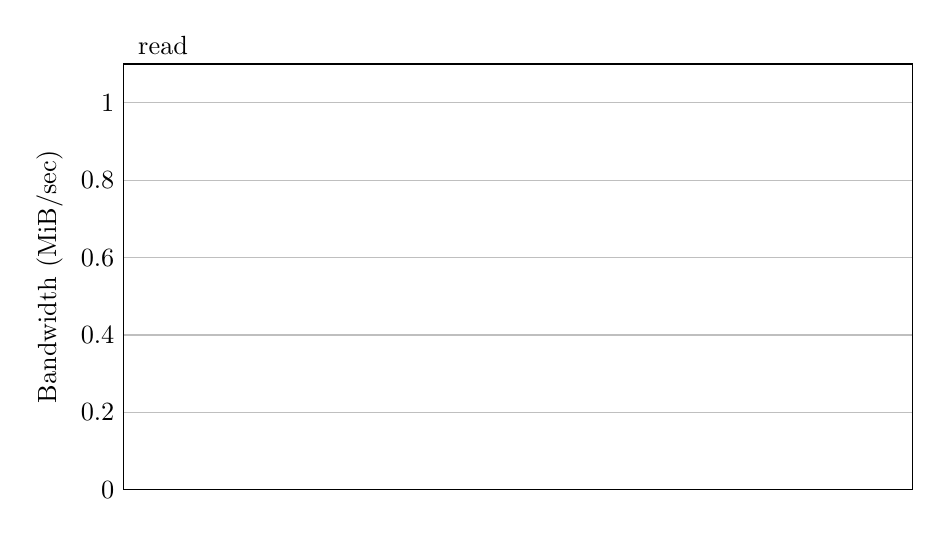
\begin{tikzpicture}[yscale=0.95, xscale=0.95]
        \begin{axis}[
                ybar,
                ymin=0,
                ylabel={Bandwidth (MiB/sec)},
                ymajorgrids=true,
                symbolic x coords={seq.write,seq.read},
                xtick={seq.write,seq.read},
                xticklabels={write,read},
                enlarge x limits=0.5,
                visualization depends on=y \as \rawy,
                xtick pos=right,
                major tick length=0in,
                xticklabel pos=right,
                nodes near coords style={font=\small,anchor=east,rotate=90,xshift=-\pgfplotsunitylength*\rawy,},
                height=.6\linewidth,
                width=\linewidth,
            ]
            \addSeqPlot{ext4};
            \addSeqPlot{btrfs};
            \addSeqPlot{xfs};
            \addSeqPlot{zfs};
            \addSeqPlot{nilfs2};
            \addSeqPlot{betrfs4};
            \addSeqPlot{betrfs5};
        \end{axis}
    \end{tikzpicture}
    \caption[Sequential-write and sequential-read benchmark]{\label{fig:seq_io}
        Bandwidth to sequentially read and write a 10 GiB file (higher is better).}
\end{figure}

Figure~\ref{fig:seq_io} shows the results.
Ext4, Btrfs, XFS performs sequential
writes close to disk bandwidth, while \betrfsFive, similar to NILFS2, is about
6.5\% slower than the fastest file system.
The performance increase of \betrfsFive from \betrfsFour is from preferential
splitting, which creates a pivot matching the maximum file data key the
beginning of the workload, avoiding further node relifting in subsequent node
splits.
For sequential reads, Ext4, Btrfs, XFS run at disk bandwidth, while \betrfsFive
is 19.1\% slower than the fastest file system, which is close to \betrfsFour
and NILFS2.
\betrfs reads a leaf, which is about 4 MiB in size, each time, while
extent-based file systems can have extents whose size is more than 100 MiB.
Thus, sequential reads results in more (and smaller) IOs on \betrfs.

\paragraph{Random writes.}

We then measure the performance of random writes on the file generated by the
sequential write benchmark.
The benchmark issues 256Ki 4-Byte overwrites (in total 1 MiB data) at random
offsets within the 10GiB file, followed by an \texttt{fsync}.

\newcolumntype{.}{D{.}{.}{-1}}

\begin{table}[t]
    \centering
    \begin{tabular}{l.@{${}\pm{}$}.}
        \hline
        File system & \multicolumn{2}{c}{random write (sec)} \\
        \hline
        \input{./data/rand_io.csv}
        \hline
    \end{tabular}
    \caption[Random-write benchmark]{\label{tab:rand_io}
        Time to perform 256Ki 4-Byte random writes one a 10GiB file (1 MiB total IO, lower is better).}
    \begin{tabular}{l.@{${}\pm{}$}..@{${}\pm{}$}..@{${}\pm{}$}.}
    \hline
    File system & \multicolumn{2}{c}{find (sec)} & \multicolumn{2}{c}{grep (sec)} & \multicolumn{2}{c}{delete (sec)} \\
    \hline
    \input{./data/dir_ops.csv}
    \hline
    \end{tabular}
    \caption[Directory operation benchmar]{\label{tab:dir_ops}
        Time to perform recursive grep, find and delete of the Linux 3.11.10 source directory (lower is better).}
\end{table}

Table~\ref{tab:rand_io} shows the results.
Because \betrfs performs upserts, which doesn't read the old data, for random
writes, performing the 1MiB random writes only takes about 5 seconds on
\betrfsFour and \betrfsFive.
However, it takes at least 2022 seconds on other file systems, which is
more than 400 times slower.

\paragraph{Directory operations.}
Next, we measure three common directory operations,
\texttt{grep}, \texttt{find}, and ``rm -rf''.
The benchmark measures the time to \texttt{grep} keyword cpu\_to\_be64 and
\texttt{find} file wait.c on a copy of the Linux 3.11.10 source directory.
Also, it measure the time to recursively delete the directory with ``rm -rf''.

Table~\ref{tab:dir_ops} shows the results.
Because full-path indexing ensures locality in \betrfs, \texttt{find} and
\texttt{grep} on \betrfsFour and \betrfsFive are more than two times faster than
other file systems.
Recursive delete is implemented by range-delete messages in \betrfsFour and
\goto messages in \betrfsFive, both shows comparable performance against other
file systems.

\paragraph{TokuBench.}

\section{Macrobenchmarks}

\section{Rename benchmarks}

\textbf{TODO}

\section{Clone benchmarks}

\textbf{TODO}

\section{Summary}


\section{Related work}
\label{sec:related}

\subsection{Write-optimized file systems}

Most write-optimized file systems are built on FUSE~\cite{fuse} and
LSM-trees~\cite{lsm}.

KVFS~\cite{kvfs} is built on VT-trees, LSM-trees with stitching.
When VT-trees flush and merge two SSTables (similar to nodes in \bets), it
identities overlapping key ranges and only merges these ranges.
This technique, which is called stitching, avoids writing the same block
multiple times but causes fragmentation.
Therefore, KVFS needs to defragment when the disk is nearly full.

TableFS~\cite{tablefs} keeps metadata and small files (less than 4KB) on the
LSM-tree and large files in the underlying ext4 file system.
Therefore, TableFS outperforms other file systems on metadata and small file
benchmarks.

TokuFS~\cite{tokufs} is a full-path indexing file system with \bets on FUSE.
It is the precursor to \betrfs, showing good performance for small writes and
directory scans.

\subsection{File systems with snapshots}

Many modern file systems provide snapshot mechanism, making read-only copies of
the whole file system.

The WAFL file system~\cite{wafl} organizes all blocks in a tree structure.
By copying the vol\_info block, which is the root of the tree structure, WAFL
creates a snapshot.
Later, WAFL introduces a level of indirection between the file system and the
underlying disks~\cite{wafl-flexvol}.
Therefore, multiple active instances of the file system can exist at the same
time and WAFL can create writable snapshots of the whole file system by creating
a new instance and copying the vol\_info block.

FFS~\cite{ffs} creates snapshots by suspending all operations and creating a
snapshot file whose inode is stored in the superblock.
The size of the snapshot file is the same as the disk.
Upon creation, most block pointers in the snapshot inode are marked
``not copied'' or ``not used'' while some metadata blocks are copied to new
addresses.
Reading a ``not copied'' address in the snapshot file results in reading the
address on the disk.
When a ``not copied'' block is modified in the file system, FFS copies the block
to a new address and updates the block pointer in the snapshot inode.

NILFS~\cite{nilfs2} is a log-structured file system that organizes all blocks
in a B-tree.
In NILFS, each logical segment contains modified blocks and a checkpoint block
used as the root of the B-tree.
NILFS gets the current view of the file system from the checkpoint block
of the last logical segment.
NILFS can create a snapshot by making a checkpoint block permanent.

ZFS~\cite{zfs} also stores the file system in a tree structure and creates
snapshots by copying the root of the tree (uberblock).
To avoid maintaining one block bitmap for each snapshot, ZFS keeps birth time
in each pointer.
A block should not be freed if its birth time is earlier than any snapshot.
In that case, the block is added to the dead list of the most recent snapshot.
When a snapshot is deleted, all blocks in its dead list are checked again before
being freed.

GCTree~\cite{gctree} implements snapshots on top of ext4.
It chains different versions of a metadata block with GCTree metadata.
Also, each pointer in the metadata block has a ``borrowed bit'' indicating
whether the target block is inherited from the previous version.
Therefore, GCTree can check whether to free a block by inspecting GCTree
metadata and doesn't need to maintain reference counts.

NOVA-Fortis~\cite{nova} targets at non-volatile main memory (NVMM).
In NOVA-Fortis, each inode has a private log with log entries pointing
to data blocks.
To enable snapshots, NOVA-Fortis keeps a global snapshot ID and adds the
creating snapshot ID to log entries in inodes.
NOVA-Fortis decides whether to free a block based on the snapshot ID in the log
entry and active snapshots.
It also deals with DAX-style \texttt{mmap} by stalling page faults when marking
all pages read-only.

\subsection{File systems with file or directory clones}

Some file systems go futher to support cloning one single directory or file.

The Episode file system~\cite{episode} groups everything under a directory into
a fileset.
Episode can create an immutable fileset clone by copying all the anodes (inodes)
and marking all block pointers in the anodes copy-on-write.
When Episode changes a block with a copy-on-write pointer, it allocates a new
block and updates the block pointer in the active fileset.

Ext3cow~\cite{ext3cow} creates immutable file clones by maintaining a
system-wide epoch and inode epochs.
When an inode is modified, ext3cow allocates a new inode if the epoch in the
inode is older than the last snapshot epoch.
Also, each directory stores birth and death epochs for each entry.
Ext3cow can render the view of the file system in a certain epoch by fetching
entries alive at that epoch.

Btrfs~\cite{btrfs} supports creating writable snapshot of the whole file system
by copying the root of the sub-volume tree in its COW friendly
B-trees~\cite{cowbtree}.
Btrfs clones a file by sharing all extents of the file.
The extent allocation tree records extents with back pointers to the inodes.
Therefore, Btrfs is able to move an extent at a later time.

\subsection{Versioning file systems}

There are also versioning file systems that versions files and directories.

EFS~\cite{efs} automatically versions files and directories.
By allocating a new inode, it creates and finalizes a new file version when the
file is opened and closed.
Each versioned file has an inode log that keeps all versions of the file.
All entries in directories have creation and deletion time.

CVFS~\cite{cvfs} tries to store metadata versions more compactly.
CVFS suggests two ways to save space in versioning file systems:
1. journal-based metadata that keeps a current version and an undo log to
recover previous versions;
2. multiversion B-trees that keep all versions of metadata in a B-tree.

Versionfs~\cite{versionfs} builds a stackable versioning file system.
Instead of building a new file system, Versionfs adds the functionality of
versioning on an existing file system by transferring certain operations to
other operations.
In this way, all versions of a file are maintained as different files in the
underlying file system.


% The graduate school Format Guide put endnotes before appendixes But the
% provided sample pages put appendixes before endnotes It's unclear which one
% is correct. Recommend to use footnotes instead of endnotes.
%\appendix
%\chapter{Example Appendix}
\label{chap:appendix}
\lipsum[1]

\chapter{Another Appendix}
\label{chap:appendix2}

\lipsum[1]

\clearpage

%\begin{center}
\vspace*{46pt}
\currentpdfbookmark{ENDNOTES}{bk:endnotes}
\textbf{ENDNOTES}
\vspace{10pt}
\end{center}
\addcontentsline{toc}{chapter}{ENDNOTES}

\theendnotes{}

\clearpage


\clearpage
\phantomsection

{\def\chapter*#1{} % suppress bibliograph header.
\begin{singlespace}
\addcontentsline{toc}{chapter}{REFERENCES}
\begin{center}
\textbf{REFERENCES}
\vspace{17pt}
\end{center}

\bibliographystyle{apalike}
\bibliography{references}
\end{singlespace}
}


\end{document}
